\section{Resultados e discussões}
\subsection{Figuras de Chladni}

\subsection{Tubo de Rijke}

\subsection{Diapasão e coluna d'água}
O experimento do diapasão com coluna de água é uma demonstração clássica da física ondulatória, utilizada para estudar os princípios da ressonância em tubos fechados. No dito experimento, ao colocar um diapasão que vibra a um frequência de \qty{512}{Hz} na boca do tubo, fez com que as ondas sonoras se propagassem pela coluna de ar dentro do tubo sendo refletido pelas paredes até a extremidade da água, que reflete a onda. 

Ao variar o nível da água no tubo por completo, ou seja, varia-lo do menor ponto até o maior ponto, foi possível observar que em dois pontos houve um grande aumento na intensidade sonora. Esses dois pontos foram marcados e tiveram suas colunas de ar medidas, como mostrado na \cref{TuboFechado}.
\begin{figure}[H]
	\centering
	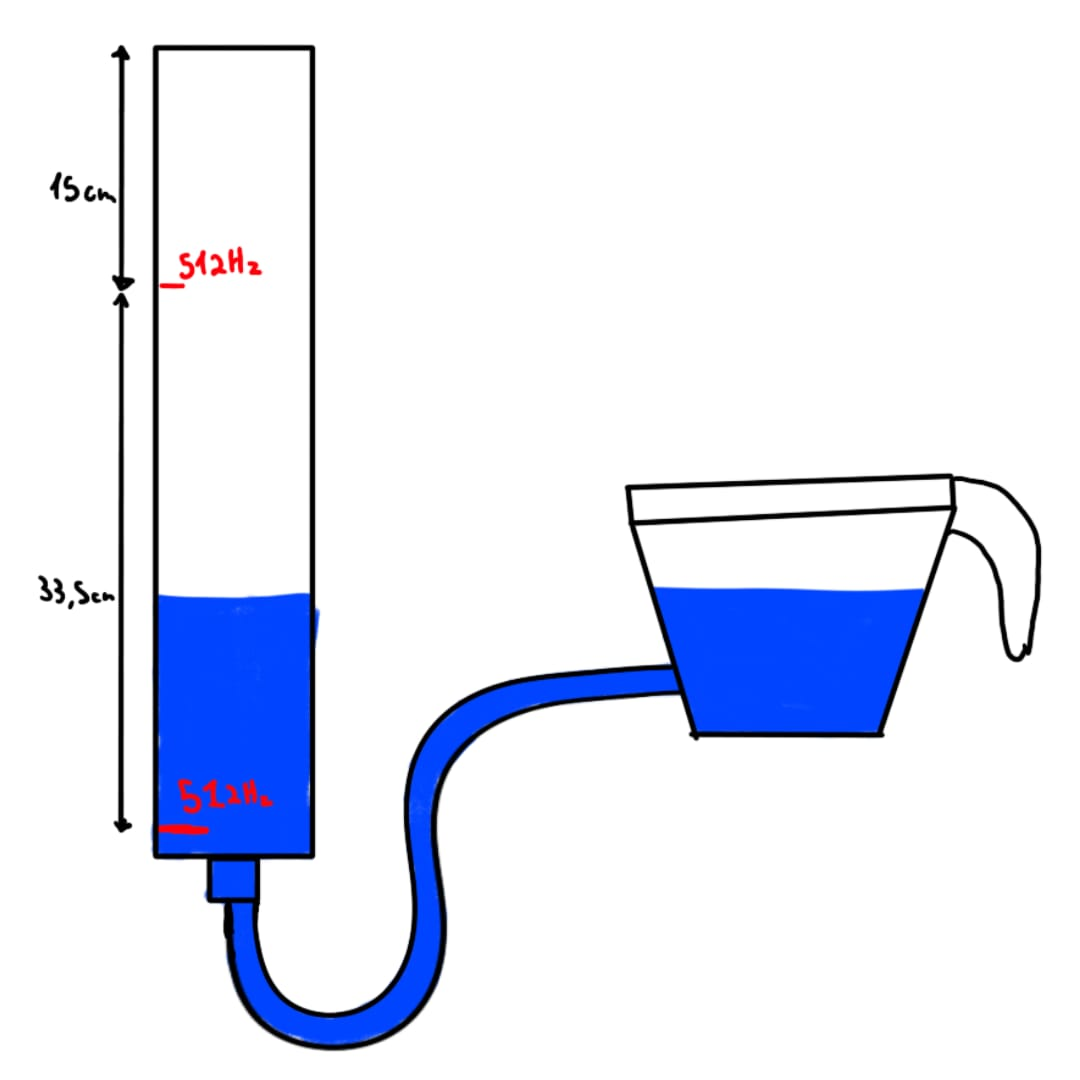
\includegraphics[width=0.35\linewidth]{fig/TuboFechado.png}
	\caption{Tubo de água com uma extremidade fechada e sistema de modificação do nível, marcados e medidos os pontos em que houveram um aumento significativo na intensidade sonora com a vibração de um diapasão de \qty{512}{Hz}. Fonte: Autoria própria}
	\label{TuboFechado}
\end{figure}

Esse aumento significativo na intensidade do som, ocorre pois quando a onda se propagou pela coluna de ar dentro do tubo, e refletiu-se pela extremidade fechada (superfície da água), criou-se uma \textit{onda refletida} com defasagem de 180º para a onda original, e essa interferência entre as ondas incidentes e refletidas deu origem a uma onda estacionária. Essas ondas estacionárias, são os modos normais de vibração da coluna de ar contida no tubo, que possuem seus pontos de ressonância identificáveis por um aumento significativo na intensidade sonora. E em um tubo com uma extremidade fechada, esses pontos de ressonância ocorrem quando o comprimento da coluna de ar (\(l\)) corresponde a múltiplos ímpares de \(\frac{\lambda}{4}\).

Segundo os dados retirados do experimento, sabe-se que os pontos de ressonância das ondas estacionarias ocorreram com uma coluna de ar de tamanhos \qty{15}{cm} e \qty{48,5}{cm}, possibilitando o calculo do comprimento da onda referente ao primeiro harmônico, que ocorre ao menor \(l\).

\begin{align*}
	l &= \frac{\lambda}{4}\\
	\qty{15}{cm} &= \frac{ \lambda}{4}\\
	\lambda &= \qty{60}{cm} = \qty{0,6}{m}
\end{align*}

Dessa forma, como possui-se o comprimento de onda do som \(\lambda\), e a frequência da onda \(f\), é possível calcular-se a velocidade do som no ar:

\begin{align*}
	v &= \lambda \cdot f\\
	v &= \qty{0,6}{m} \cdot \qty{512}{Hz} \\
	v &= \qty{307,2}{m/s}
\end{align*}

Os resultados experimentais indicaram uma velocidade do som de \qty{307,2}{m/s}, apresentando uma diferença de aproximadamente 10,4\% em relação ao valor teórico de \qty{343}{m/s}. Esta discrepância pode ser atribuída principalmente a: (1) variações nas condições ambientais (temperatura e umidade), já que a velocidade do som varia com a temperatura do ar; (2) imprecisões na determinação do ponto exato de ressonância; e (3) possíveis erros sistemáticos nas medições. Apesar da diferença, o experimento demonstrou ser um método válido para estimativa da velocidade do som em condições controladas.

\subsection{Experimento de Uma Corda}
Este experimento ilustra o princípio de funcionamento dos instrumentos de corda, nos quais o som é produzido pela vibração das cordas. Ao serem colocadas em oscilação, as cordas perturbam o meio ao seu redor, gerando ondas sonoras — variações de pressão que se propagam pelo ar. O perfil dessa oscilação determina as características da onda sonora gerada. Assim, ao alterar propriedades como a frequência ou o comprimento da corda, modifica-se o som produzido.

No experimento de uma corda, observou-se a variação do som emitido pela vibração da corda ao alterar a tensão da mesma. A explicação dessa alteração de som é sustentada pelas leis das Cordas Vibrantes, descritas por Mersenne, e englobadas na seguinte expressão:
\begin{align*}
	v_1 = \frac{1}{2l} \sqrt{\frac{T}{\mu}}
\end{align*}
Sendo \(v_1\) a frequência fundamental, \(l\) o comprimento da corda, \(T\) e  \( \mu\), a Tensão da corda e sua Densidade linear de massa.
A partir dessa expressão, é possível retirar as três leis de Mersenne. Tais que, a frequência fundamental é: (i) inversamente proporcional ao comprimento da corda; (ii) proporcional à raiz quadrada da tensão; (iii) inversamente proporcional à raiz quadrada da densidade linear de massa da corda. Demonstrando, com a segunda lei, o porquê ao variar a tensão da corda houve uma alteração no som.

Essas leis também explicam por que, nos instrumentos de corda, a modificação do som pode ser feita pela variação da tensão das cordas ou pela utilização de cordas diferentes. Como o comprimento da corda é limitado pelo tamanho do instrumento, e a tensão máxima é restringida pela resistência do material, uma alternativa viável é recorrer à terceira lei, que envolve a densidade linear de massa da corda. Alterando-se esse parâmetro — ou seja, utilizando cordas com diferentes espessuras e materiais — é possível ampliar a gama de sons produzidos por um mesmo instrumento. Esse princípio é claramente observado nas guitarras, em que cada corda possui uma espessura distinta e, por isso, emite sons diferentes.
